% Chapter 6 section 6.3: results -- 6.3.1 overview and 6.3.2, written 2026-09-26.
% Drafted in the chat and approved before this write (CLAUDE.md §2 steps 5-6).
% Structure fixed 2026-09-26 (Abram), manifest §9b row 6.3: an overview and THREE experiments.
%   6.3.1 overview
%   6.3.2 What the retrieved context changes        -> H2.1, H2.2   [written]
%   6.3.3 whether better retrieval reaches the answer -> H2.3, H2.4 [to come: one scatter,
%         two y axes, Kendall's tau on each, no p-value]
%   6.3.4 generator size, answering RQ3             -> H3.1         [to come: ten pairs, not
%         105, said once; cross-size ordering as an observation with no verdict]
% The oracle ceiling is NOT reported (manifest §9b, 2026-09-26). No depth sweep (2026-09-19).
% Every number here is manifest §14 R9 (registered 2026-09-26, O-23 closed). NO R8 figure.
% Headings name what is studied: no hypothesis ID and no verdict in a heading (CLAUDE.md §5).
% No numbered subheadings inside a subsection -- bold lead-ins (manifest §4b).
% No 0.02 limit in this chapter: it is the relevance judge's and governs retrieval scores
%   alone (§6.1). No test, no interval, no "significant" (manifest §1c-i).
% The verdicts are §6.4's. This section says which rule each hypothesis reads and stops.
% §6.4 landed 2026-09-26: the three placeholders are now \ref{sec:gen-verdicts}.
% Float: [!t] deliberately. Table 6.1 and Figure 6.1 are already queued in §6.2, and one table
%   that cannot be placed defers every later table in the chapter, silently (manifest §15).

% ⚠ WORDING REPAIRED 2026-09-27 (Abram), with the §7.1 write. SLT-TYPE's answers are "nonetheless
%   NOT DRAGGED BELOW the floor, at 0.196", not "nonetheless above the floor". A per-topic check of
%   the 1.5B per-sample score files (DIAGNOSTIC ONLY -- not registered, not reportable, not citable)
%   shows the 0.196-against-0.170 gap is five topics rescued from zero factual correctness, with a
%   median per-topic difference of 0.000, so "above the floor" states a five-topic tail as a level.
%   §6.4 carries the matching repair and §7.1 uses the same words. UNCHANGED deliberately: the
%   ten-above / five-below count earlier in this subsection and §6.3.3's "stands above eight of the
%   fourteen" -- both are counts over the reported means, not causal claims, and three sections
%   argue from them. Snapshot `_sec63_results.preFloorWording.bak.tex`.
\section{Results}\label{sec:gen-results}

\subsection{Overview}\label{sec:gen-res-intro}

Three experiments answer the questions this chapter asks, and they run in the order the
argument needs. The first two change what the generator is given and hold everything else
fixed: whether a retrieved context reaches the answer at all, and then whether a better
context reaches it further. The third changes the generator rather than the context,
repeating both at three and at seven billion parameters.

% --------------------------------------------------------------------------------------------
\subsection{What the retrieved context changes}\label{sec:gen-res-context}

A retrieval system that ranks better does not thereby produce a better answer. The generator
may ignore what it is given, or use it and be carried wrong by it, and nothing in
Chapter~\ref{ch:retrieval} says which happens. This section puts three settings beside one
another on the 1.5-billion-parameter generator: no context at all, the context of the
strongest text-only retrieval, and the context of the multi-index retriever. One template
serves all three, so what separates them is the context.

Two hypotheses read these answers. Hypothesis H2.1 predicts that the multi-index retriever's
context makes answers more factually correct than generation without retrieval, and holds only
if the blocked system is ahead of the floor on FC-P. Hypothesis H2.2 predicts that the same
context makes answers both more factually correct and more faithful than the strongest
text-only retrieval's, and holds only if the blocked system is ahead of dense retrieval on
both measures. Neither reads a threshold: the values are read as they are reported.

\textbf{Against no context.} The floor reaches 0.170 FC-P over the 78 topics of
Section~\ref{sec:met-collection} and the blocked system 0.206, ahead by 0.036
(Table~\ref{tab:gen-res-context}). It is ahead on 33 of the 78 topics, behind on 23 and level
on 22; the scoring framework rounds each factual-correctness score to two decimals, which is
why so many topics come out level. Section~\ref{sec:gen-verdicts} rules on H2.1.

The floor is not the bottom of the field, though. Ten of the fifteen configurations of
Section~\ref{sec:met-retrieval-configs} stand above it on FC-P and five below --- OPT, SLT,
the formula block, dense with SLT-TYPE, and dense with the three formula rankings each voting
separately. A retrieved context is therefore not an improvement in itself. Below some level of
retrieval quality the answers built from a context are worse than answers written from none.

The one configuration that breaks the pattern marks what drives it. SLT-TYPE alone is the
weakest retrieval of the fifteen and its answers are nonetheless not dragged below the floor,
at 0.196, while their faithfulness is the lowest in the chapter at 0.049 --- almost nothing they say
comes from the context (Figure~\ref{fig:gen-res-tau}). Each of the five that fall below the floor draws on its context more
than that. A context weak enough to be ignored costs the generator nothing, and a context used
but wrong costs it the answer.

\textbf{Against the strongest text-only retrieval.} Section~\ref{sec:ret-verdicts} found the
two systems indistinguishable as retrieval, 0.551 against dense retrieval's 0.557 on
nDCG$'$@10. Their answers are not indistinguishable. On faithfulness the blocked system is
ahead, 0.189 against 0.171, and ahead on 37 topics against 33; on FC-P it is behind, 0.206
against 0.241, and behind on 39 topics against 24. H2.2 needs both, so the correctness half
decides it, and Section~\ref{sec:gen-verdicts} rules on it.

The two measures answer different questions, as Section~\ref{sec:gen-overview} set out, and
here they answer in opposite directions. More of what the generator says under the multi-index
context is traceable to that context, and less of what it says is right. The multi-index
context is used more and helps less.

Two comparisons read two points each, and the field has fifteen. Whether where a context sits
in the retrieval ordering predicts anything about the answers built from it is the question
the next section asks of all fifteen at once.

\begin{table}[!t]
\centering
\small
\renewcommand{\arraystretch}{1.15}
\begin{tabular}{lrrr}
\toprule
Context & nDCG$'$@10 & Faithfulness & FC-P \\
\midrule
No context --- the floor & ---   & ---   & 0.170 \\
Dense retrieval          & 0.557 & 0.171 & \textbf{0.241} \\
Blocked multi-index      & 0.551 & \textbf{0.189} & 0.206 \\
\bottomrule
\end{tabular}
\caption[What the retrieved context changes]{Answers generated without a context, from dense retrieval's context, and from the
blocked multi-index retriever's. \emph{nDCG$'$@10}: prime normalised discounted cumulative
gain at rank 10, the retrieval quality of Chapter~\ref{ch:retrieval}. \emph{FC-P}:
factual-correctness precision. Faithfulness is undefined without a context. The 78 topics of
Section~\ref{sec:met-collection}, five retrieved answers as context, 1.5-billion-parameter
generator. The highest value in each of the two answer-quality columns is set in bold.}
\label{tab:gen-res-context}
\end{table}

% --------------------------------------------------------------------------------------------
% 6.3.3 written 2026-09-26, drafted in the chat over two passes and approved before this write.
% Vocabulary is §3.6's own: two ORDERINGS of the same systems, CONCORDANT and DISCORDANT pairs.
%   The word "association" is deliberately not used here (§6.2 still carries it twice -- sweep
%   together or leave, Abram's call, raised 2026-09-26).
% Numbers: manifest §14 R9.B, including the discordance breakdown registered the same day.
%   NO SUBSET TAU is computed or reported -- the rules read all 105 pairs and a coefficient over
%   a chosen subset would be a re-fit (CLAUDE.md §5).
% Cut on Abram's instruction, 2026-09-26: the closing caution paragraph (that the two values
%   describe the fifteen taken together and say nothing about a small gain at the top of the
%   range, with dense vs blocked as the case in point).
% Figure 6.2 added 2026-09-26 (Abram's choice, shown in the chat): TWO PANELS sharing the x axis,
%   not the two y axes manifest §9b specifies -- on one pair of axes the two clouds overlap and the
%   eye compares heights measured against different scales. Both series are round markers, the
%   chapter's two blues. Generated by experiments/diagnostics/plot_generation_tau_figure.py, which
%   recomputes both tau from the per-answer score files and reproduces R9's values exactly.
%   ONE \ref only, at the result sentence -- Abram's instruction, references only where needed.
% §6.4 landed 2026-09-26: the three placeholders are now \ref{sec:gen-verdicts}.

\subsection{Retrieval quality and answer quality}\label{sec:gen-res-tau}

% Float placement: declared HERE, immediately after the heading, not at the end of the
%   subsection. A [t] float can only reach the top of a page LATER than its declaration
%   point, so declared at the end of §6.3.3 -- which sat on page 73 -- it was deferred to
%   page 74. Declared at the head of §6.3.3, while the page is still 72, the first top it
%   can reach is page 73. [!t] waives the placement fractions for this float alone
%   (manifest §15 float-discipline note). Figures queue separately from tables, so Table 6.2
%   is unaffected. Re-check the page numbers in ausarbeitung.aux after the build, not by eye.
\begin{figure}[!t]
\centering
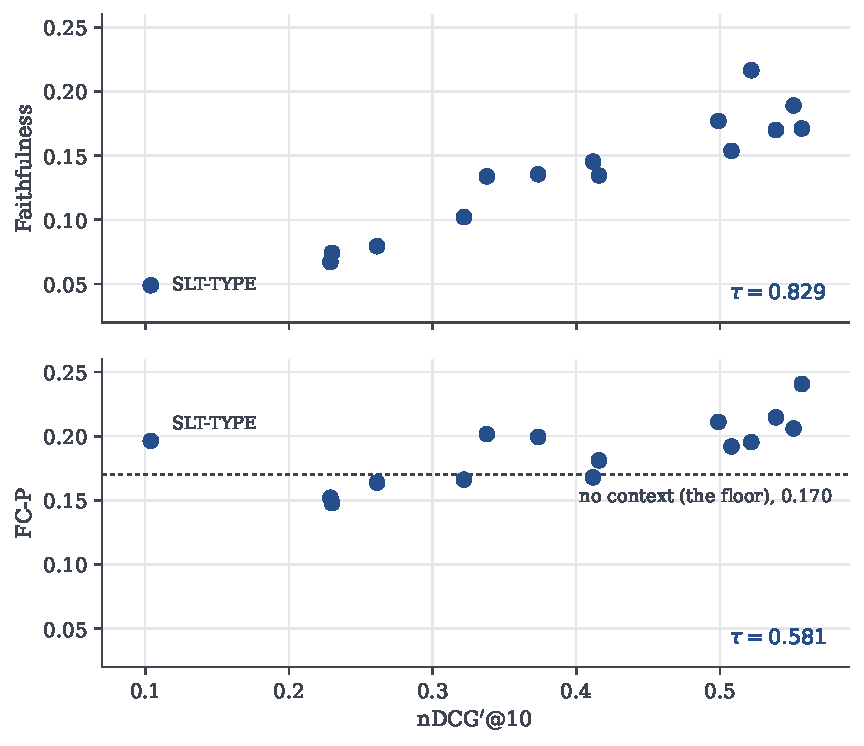
\includegraphics[width=0.82\textwidth]{images/gen_tau_retrieval_quality.pdf}
\caption[Answer quality against retrieval quality]{Faithfulness and factual-correctness precision (FC-P) of the generated answers, against
the retrieval quality of the configuration that supplied the context, over the fifteen
configurations of Section~\ref{sec:met-retrieval-configs}. Kendall's $\tau$ in each panel, over
all 105 pairs. The dashed line marks generation without retrieval, which has an FC-P but no
faithfulness and so appears in the lower panel alone. SLT-TYPE is named in both panels as the
configuration the surrounding text argues from. \emph{nDCG$'$@10}: prime normalised discounted
cumulative gain at rank 10, under the judge labels. The 78 topics of
Section~\ref{sec:met-collection}, five retrieved answers as context, 1.5-billion-parameter
generator.}
\label{fig:gen-res-tau}
\end{figure}

The two comparisons of Section~\ref{sec:gen-res-context} each read a pair of systems, and a pair
cannot say whether the relation holds in general: two systems may differ for reasons that have
nothing to do with how well either retrieved. The fifteen configurations can answer it, because
they retrieve at very different levels --- from 0.104 to 0.557 nDCG$'$@10.

Two hypotheses put the question, one for each measure. Hypothesis H2.3 predicts that faithfulness
rises with the quality of the retrieved context: the better the context, the more of the answer
comes from it. Hypothesis H2.4 predicts the same of factual correctness. Each is rejected if its
measure does not rise with retrieval quality across the fifteen. Every pair enters the Kendall's
$\tau$, and no resolving power is applied to it: the 0.02 of
Section~\ref{sec:met-judge-validation} sets no pair aside as too close to order.

Both measures rise with retrieval quality (Figure~\ref{fig:gen-res-tau}). Ordering the fifteen by retrieval quality and again by
faithfulness leaves the two orderings concordant on 96 of the 105 pairs, $\tau = 0.829$. Ordering
them by factual correctness instead leaves 83 of 105 concordant, $\tau = 0.581$. The closing
section of this chapter rules on H2.3 and H2.4.

Read together, the two say more than either does alone. The generator draws on the context it is
given, and the better that context, the more of the answer comes from it: only 9 of the 105 pairs
run the other way. Correctness rises too, and less evenly, with 22 pairs out of order. The chain
from retrieval to the answer has two links and they are not equally tight. A better context is
more likely to be used, and being used is not the same as being right.

Where correctness runs backwards is worth naming. Eight of its 22 discordant pairs involve
SLT-TYPE alone. It retrieves worst of the fifteen and its faithfulness is the lowest in the
chapter, 0.049, so the generator hardly touches what it supplies and writes much the same answer
it would write from no context at all. At 0.196 that answer stands above eight of the fourteen
configurations that retrieve better than it does (Figure~\ref{fig:gen-res-tau}). A context the generator does not use cannot pull
its answers down to the level of the retrieval behind it.

Both orderings are read on the smallest generator, on the same fifteen contexts throughout.
Whether either survives a larger one is the last question this chapter asks.

% --------------------------------------------------------------------------------------------
% 6.3.4 written 2026-09-26, drafted in the chat and approved before this write.
% Answers RQ3 and rules on nothing -- H3.1's verdict is §6.4's.
% Numbers: manifest §14 R9.C, including the below-floor counts registered the same day.
% Carries, as manifest §9b requires: RQ2.1's two comparisons repeated at each size; both measures
%   against retrieval quality over the five common conditions; the 1.5B value over those same five
%   as a REFERENCE POINT, not a test; the ten-pairs-against-105 caveat, stated once, as the reason
%   rather than the rule (§6.2 carries the comparability rule itself); and the cross-size ordering
%   as an OBSERVATION WITH NO VERDICT.
% ⚠ H3.1's CLAUSE (a) WAS RESTATED 2026-09-26 (Abram) and this section is written against the
%   restated wording: at 3B and 7B each of RQ2.1's three comparisons must run in the SAME DIRECTION
%   as at 1.5B. The rule drafted 2026-09-24 read absolute directions -- blocked ahead of dense on
%   BOTH measures -- which had operationalised the prior-form statement on the assumption that H2.2
%   would be supported; H2.2 was not, so that rule had become a restatement of H2.2's failed
%   condition and failed at all three sizes for a reason unrelated to generator size. Full note and
%   the disclosure in manifest §1c and §10 (the §7.2 post-hoc row).
%   THE VERDICT DOES NOT MOVE -- not supported either way: clause (b) fails at 3B on its own
%   (FC-P tau = 0.000) and clause (a) now fails at 7B. §6.4 must say that RQ2.1 REPLICATES AT 3B
%   and breaks at 7B, not that the experiment failed everywhere. This section states the directions
%   and rules on nothing.
% Float: Table 6.3 declared at the head of the subsection, not at its end -- a [!t] float can only
%   reach the top of a page LATER than its declaration point, which is what put Figure 6.2 a page
%   late. Tables queue in declaration order behind Tables 6.1 and 6.2; re-check every later table
%   in the chapter on the build, from ausarbeitung.aux (manifest §15 float-discipline note).

\subsection{The size of the generator}\label{sec:gen-res-sizes}

\begin{table}[!t]
\centering
\small
\setlength{\tabcolsep}{4.5pt}
\renewcommand{\arraystretch}{1.15}
\begin{tabular}{lrrrrrrr}
\toprule
& & \multicolumn{2}{c}{1.5B} & \multicolumn{2}{c}{3B} & \multicolumn{2}{c}{7B} \\
\cmidrule(lr){3-4}\cmidrule(lr){5-6}\cmidrule(lr){7-8}
Context & nDCG$'$@10 & Faith. & FC-P & Faith. & FC-P & Faith. & FC-P \\
\midrule
No context --- the floor & ---   & ---   & 0.170 & ---   & 0.201 & ---   & 0.246 \\
\addlinespace
formula block            & 0.261 & 0.079 & 0.164 & 0.072 & 0.214 & 0.086 & 0.229 \\
BM25                     & 0.338 & 0.134 & 0.202 & 0.150 & 0.214 & 0.162 & 0.243 \\
BM25 + dense             & 0.539 & 0.170 & 0.215 & 0.174 & 0.204 & \textbf{0.225} & 0.272 \\
blocked                  & 0.551 & \textbf{0.189} & 0.206 & \textbf{0.214} & 0.214 & 0.197 & \textbf{0.281} \\
dense                    & 0.557 & 0.171 & \textbf{0.241} & 0.189 & \textbf{0.313} & 0.221 & 0.277 \\
\bottomrule
\end{tabular}
\caption[The three generator sizes]{The floor and the five configurations generated at all three generator sizes, ordered by
retrieval quality. \emph{Faith.}: faithfulness, undefined without a context. \emph{FC-P}:
factual-correctness precision. \emph{nDCG$'$@10}: prime normalised discounted cumulative gain at
rank 10, under the judge labels. \emph{1.5B}, \emph{3B}, \emph{7B}: generators of 1.5, 3 and 7
billion parameters. The 78 topics of Section~\ref{sec:met-collection}, five retrieved answers as
context. The highest value in each faithfulness and FC-P column is set in bold; the nDCG$'$@10
column orders the rows and is not marked.}
\label{tab:gen-res-sizes}
\end{table}

Everything so far is read on a 1.5-billion-parameter generator, the smallest of the three. A model
that size has less of its own to bring, so a retrieved context has more room to matter to it, and a
larger model may need it less. The third research question asks whether the answers to the second
survive that change. It is a sanity check on those answers rather than a question about generators
in their own right.

The floor and five of the fifteen configurations --- the two text indexes, their fusion, the formula
block and the blocked system --- were generated again at 3 and at 7 billion parameters, with the
prompt, the context size, the decoding and the topics all held fixed
(Table~\ref{tab:gen-res-sizes}). Hypothesis H3.1 predicts that the conclusions of the second
research question are not specific to the smallest generator, in two clauses. The first asks that
each of the three comparisons of Section~\ref{sec:gen-res-context} --- the blocked system against
the floor on FC-P, and against dense retrieval on FC-P and on faithfulness --- runs in the same
direction at the larger sizes as it does at the smallest. The second asks that both measures still
rise with retrieval quality there.

\textbf{The three comparisons at each size.} All three keep their direction at 3 billion
parameters; two of them reverse at 7 billion. Against the floor, the blocked system stays ahead on
FC-P throughout: 0.206 against 0.170 at 1.5 billion parameters, 0.214 against 0.201 at 3 billion
and 0.281 against 0.246 at 7 billion. That is the direction
Section~\ref{sec:gen-res-context} found, and both larger generators keep it. Against dense
retrieval the blocked system is behind on FC-P at the two smaller sizes, 0.206 against 0.241 and
0.214 against 0.313, and ahead at the largest, 0.281 against 0.277; on faithfulness it runs the
other way, ahead at the two smaller sizes, 0.189 against 0.171 and 0.214 against 0.189, and behind
at the largest, 0.197 against 0.221. Both of these match
Section~\ref{sec:gen-res-context} at 3 billion parameters and reverse at 7 billion. The two
reversals run in opposite senses: under the largest generator the blocked system's context produces
the more factually correct answers of the two, and supplies less of what those answers say.

\textbf{Retrieval quality at each size.} Over the five conditions common to all three sizes,
faithfulness rises with retrieval quality at every size: $\tau = 0.800$ at 1.5 billion parameters,
0.800 at 3 billion and 0.600 at 7 billion. Factual correctness rises at the smallest and the
largest, $\tau = 0.800$ in both, and at 3 billion it does not, $\tau = 0.000$, with five of the ten
pairs in one order and five in the other. The value at 1.5 billion is a reference point rather than
a test --- the clause reads the two larger sizes, and computing the same $\tau$ over the same
five conditions puts all three sizes on one instrument. All three are read over ten pairs where
Section~\ref{sec:gen-res-tau} reads 105, so a single pair changing places moves one of them by
0.200; they may be set beside each other and beside nothing else. Section~\ref{sec:gen-verdicts} rules on H3.1.

\textbf{What the ladder shows about generators.} One thing more is worth recording, and it
decides nothing. The floor's FC-P rises at every step in generator size: 0.170 at 1.5 billion
parameters, 0.201 at 3 billion and 0.246 at 7 billion. At 1.5 billion it stands above one of the
five conditions, at 3 billion above none, and at 7 billion above two --- BM25 at 0.243 and the
formula block at 0.229, against its own 0.246. Answers built from those two contexts are less
factually correct than answers built from no context at all. The larger the generator, the more of
the answer it already holds, and the better a retrieved context has to be before it adds anything.
